% Created by tikzDevice version 0.10.1 on 2020-02-15 15:54:51
% !TEX encoding = UTF-8 Unicode
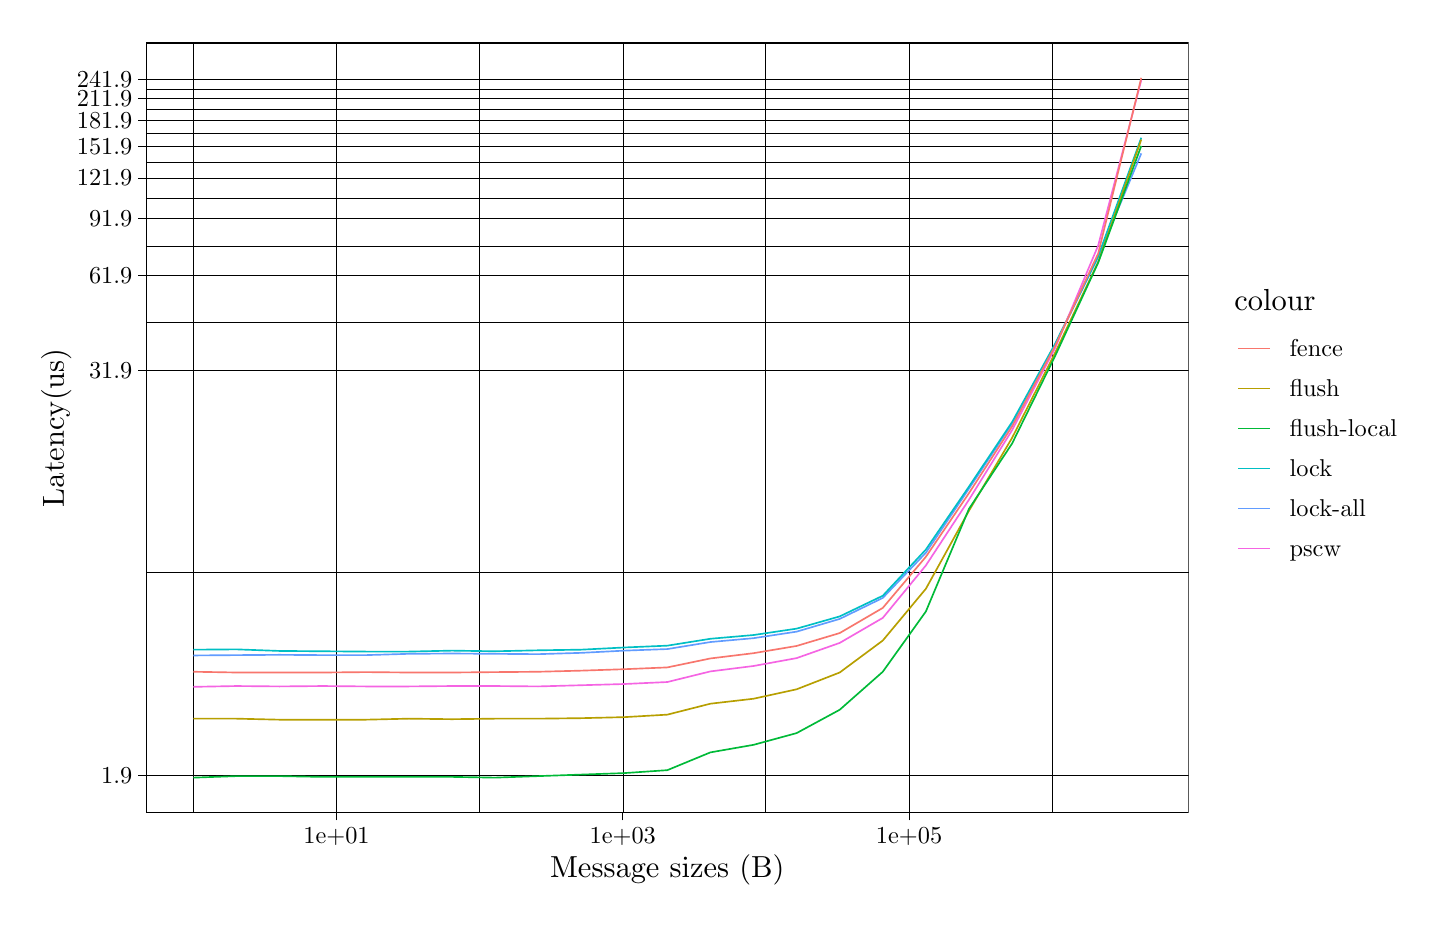
\begin{tikzpicture}[x=1pt,y=1pt]
\definecolor{fillColor}{RGB}{255,255,255}
\path[use as bounding box,fill=fillColor,fill opacity=0.00] (0,0) rectangle (505.89,314.37);
\begin{scope}
\path[clip] (  0.00,  0.00) rectangle (505.89,314.37);
\definecolor{drawColor}{RGB}{255,255,255}
\definecolor{fillColor}{RGB}{255,255,255}

\path[draw=drawColor,line width= 0.6pt,line join=round,line cap=round,fill=fillColor] (  0.00,  0.00) rectangle (505.89,314.37);
\end{scope}
\begin{scope}
\path[clip] ( 42.76, 30.72) rectangle (419.53,308.87);
\definecolor{fillColor}{RGB}{255,255,255}

\path[fill=fillColor] ( 42.76, 30.72) rectangle (419.53,308.87);
\definecolor{drawColor}{RGB}{0,0,0}

\path[draw=drawColor,line width= 0.0pt,line join=round] ( 42.76,117.35) --
	(419.53,117.35);

\path[draw=drawColor,line width= 0.0pt,line join=round] ( 42.76,207.71) --
	(419.53,207.71);

\path[draw=drawColor,line width= 0.0pt,line join=round] ( 42.76,235.15) --
	(419.53,235.15);

\path[draw=drawColor,line width= 0.0pt,line join=round] ( 42.76,252.72) --
	(419.53,252.72);

\path[draw=drawColor,line width= 0.0pt,line join=round] ( 42.76,265.76) --
	(419.53,265.76);

\path[draw=drawColor,line width= 0.0pt,line join=round] ( 42.76,276.14) --
	(419.53,276.14);

\path[draw=drawColor,line width= 0.0pt,line join=round] ( 42.76,284.77) --
	(419.53,284.77);

\path[draw=drawColor,line width= 0.0pt,line join=round] ( 42.76,292.17) --
	(419.53,292.17);

\path[draw=drawColor,line width= 0.0pt,line join=round] ( 59.89, 30.72) --
	( 59.89,308.87);

\path[draw=drawColor,line width= 0.0pt,line join=round] (163.32, 30.72) --
	(163.32,308.87);

\path[draw=drawColor,line width= 0.0pt,line join=round] (266.76, 30.72) --
	(266.76,308.87);

\path[draw=drawColor,line width= 0.0pt,line join=round] (370.20, 30.72) --
	(370.20,308.87);

\path[draw=drawColor,line width= 0.1pt,line join=round] ( 42.76, 44.19) --
	(419.53, 44.19);

\path[draw=drawColor,line width= 0.1pt,line join=round] ( 42.76,190.51) --
	(419.53,190.51);

\path[draw=drawColor,line width= 0.1pt,line join=round] ( 42.76,224.90) --
	(419.53,224.90);

\path[draw=drawColor,line width= 0.1pt,line join=round] ( 42.76,245.40) --
	(419.53,245.40);

\path[draw=drawColor,line width= 0.1pt,line join=round] ( 42.76,260.05) --
	(419.53,260.05);

\path[draw=drawColor,line width= 0.1pt,line join=round] ( 42.76,271.46) --
	(419.53,271.46);

\path[draw=drawColor,line width= 0.1pt,line join=round] ( 42.76,280.81) --
	(419.53,280.81);

\path[draw=drawColor,line width= 0.1pt,line join=round] ( 42.76,288.73) --
	(419.53,288.73);

\path[draw=drawColor,line width= 0.1pt,line join=round] ( 42.76,295.60) --
	(419.53,295.60);

\path[draw=drawColor,line width= 0.1pt,line join=round] (111.60, 30.72) --
	(111.60,308.87);

\path[draw=drawColor,line width= 0.1pt,line join=round] (215.04, 30.72) --
	(215.04,308.87);

\path[draw=drawColor,line width= 0.1pt,line join=round] (318.48, 30.72) --
	(318.48,308.87);
\definecolor{drawColor}{RGB}{97,156,255}

\path[draw=drawColor,line width= 0.6pt,line join=round] ( 59.89, 87.52) --
	( 75.45, 87.64) --
	( 91.02, 87.75) --
	(106.59, 87.64) --
	(122.16, 87.64) --
	(137.73, 88.11) --
	(153.30, 88.22) --
	(168.87, 88.11) --
	(184.44, 87.99) --
	(200.01, 88.46) --
	(215.58, 89.26) --
	(231.14, 89.83) --
	(246.71, 92.37) --
	(262.28, 93.76) --
	(277.85, 96.12) --
	(293.42,100.72) --
	(308.99,108.31) --
	(324.56,124.64) --
	(340.13,147.79) --
	(355.70,171.26) --
	(371.27,199.78) --
	(386.83,231.54) --
	(402.40,268.94);
\definecolor{drawColor}{RGB}{0,191,196}

\path[draw=drawColor,line width= 0.6pt,line join=round] ( 59.89, 89.61) --
	( 75.45, 89.72) --
	( 91.02, 89.15) --
	(106.59, 89.03) --
	(122.16, 88.92) --
	(137.73, 88.92) --
	(153.30, 89.26) --
	(168.87, 89.03) --
	(184.44, 89.38) --
	(200.01, 89.61) --
	(215.58, 90.40) --
	(231.14, 91.06) --
	(246.71, 93.55) --
	(262.28, 94.90) --
	(277.85, 97.21) --
	(293.42,101.63) --
	(308.99,109.10) --
	(324.56,125.79) --
	(340.13,148.53) --
	(355.70,171.82) --
	(371.27,200.17) --
	(386.83,231.76) --
	(402.40,274.59);
\definecolor{drawColor}{RGB}{183,159,0}

\path[draw=drawColor,line width= 0.6pt,line join=round] ( 59.89, 64.68) --
	( 75.45, 64.68) --
	( 91.02, 64.31) --
	(106.59, 64.31) --
	(122.16, 64.31) --
	(137.73, 64.68) --
	(153.30, 64.49) --
	(168.87, 64.68) --
	(184.44, 64.68) --
	(200.01, 64.86) --
	(215.58, 65.23) --
	(231.14, 66.13) --
	(246.71, 70.09) --
	(262.28, 71.88) --
	(277.85, 75.29) --
	(293.42, 81.36) --
	(308.99, 92.91) --
	(324.56,111.61) --
	(340.13,139.80) --
	(355.70,166.11) --
	(371.27,196.88) --
	(386.83,229.73) --
	(402.40,273.94);
\definecolor{drawColor}{RGB}{0,186,56}

\path[draw=drawColor,line width= 0.6pt,line join=round] ( 59.89, 43.37) --
	( 75.45, 43.92) --
	( 91.02, 43.92) --
	(106.59, 43.64) --
	(122.16, 43.64) --
	(137.73, 43.64) --
	(153.30, 43.64) --
	(168.87, 43.37) --
	(184.44, 43.92) --
	(200.01, 44.47) --
	(215.58, 45.01) --
	(231.14, 46.07) --
	(246.71, 52.50) --
	(262.28, 55.22) --
	(277.85, 59.46) --
	(293.42, 67.89) --
	(308.99, 81.63) --
	(324.56,103.41) --
	(340.13,140.48) --
	(355.70,164.07) --
	(371.27,195.74) --
	(386.83,229.45) --
	(402.40,271.66);
\definecolor{drawColor}{RGB}{245,100,227}

\path[draw=drawColor,line width= 0.6pt,line join=round] ( 59.89, 76.18) --
	( 75.45, 76.47) --
	( 91.02, 76.33) --
	(106.59, 76.47) --
	(122.16, 76.33) --
	(137.73, 76.33) --
	(153.30, 76.47) --
	(168.87, 76.47) --
	(184.44, 76.33) --
	(200.01, 76.76) --
	(215.58, 77.20) --
	(231.14, 77.92) --
	(246.71, 81.76) --
	(262.28, 83.71) --
	(277.85, 86.56) --
	(293.42, 92.05) --
	(308.99,101.09) --
	(324.56,120.04) --
	(340.13,143.79) --
	(355.70,168.90) --
	(371.27,198.62) --
	(386.83,235.67) --
	(402.40,295.41);
\definecolor{drawColor}{RGB}{248,118,109}

\path[draw=drawColor,line width= 0.6pt,line join=round] ( 59.89, 81.63) --
	( 75.45, 81.36) --
	( 91.02, 81.36) --
	(106.59, 81.36) --
	(122.16, 81.50) --
	(137.73, 81.36) --
	(153.30, 81.36) --
	(168.87, 81.50) --
	(184.44, 81.63) --
	(200.01, 82.03) --
	(215.58, 82.55) --
	(231.14, 83.20) --
	(246.71, 86.44) --
	(262.28, 88.34) --
	(277.85, 90.95) --
	(293.42, 95.61) --
	(308.99,104.70) --
	(324.56,123.17) --
	(340.13,146.17) --
	(355.70,170.26) --
	(371.27,199.38) --
	(386.83,232.79) --
	(402.40,296.23);
\definecolor{drawColor}{RGB}{0,0,0}

\path[draw=drawColor,line width= 0.6pt,line join=round,line cap=round] ( 42.76, 30.72) rectangle (419.53,308.87);
\end{scope}
\begin{scope}
\path[clip] (  0.00,  0.00) rectangle (505.89,314.37);
\definecolor{drawColor}{RGB}{0,0,0}

\node[text=drawColor,anchor=base west,inner sep=0pt, outer sep=0pt, scale=  0.88] at ( 26.57, 41.37) {1.9};

\node[text=drawColor,anchor=base west,inner sep=0pt, outer sep=0pt, scale=  0.88] at ( 22.17,187.69) {31.9};

\node[text=drawColor,anchor=base west,inner sep=0pt, outer sep=0pt, scale=  0.88] at ( 22.17,222.08) {61.9};

\node[text=drawColor,anchor=base west,inner sep=0pt, outer sep=0pt, scale=  0.88] at ( 22.17,242.57) {91.9};

\node[text=drawColor,anchor=base west,inner sep=0pt, outer sep=0pt, scale=  0.88] at ( 17.77,257.23) {121.9};

\node[text=drawColor,anchor=base west,inner sep=0pt, outer sep=0pt, scale=  0.88] at ( 17.77,268.64) {151.9};

\node[text=drawColor,anchor=base west,inner sep=0pt, outer sep=0pt, scale=  0.88] at ( 17.77,277.99) {181.9};

\node[text=drawColor,anchor=base west,inner sep=0pt, outer sep=0pt, scale=  0.88] at ( 17.77,285.91) {211.9};

\node[text=drawColor,anchor=base west,inner sep=0pt, outer sep=0pt, scale=  0.88] at ( 17.77,292.78) {241.9};
\end{scope}
\begin{scope}
\path[clip] (  0.00,  0.00) rectangle (505.89,314.37);
\definecolor{drawColor}{RGB}{0,0,0}

\path[draw=drawColor,line width= 0.3pt,line join=round] ( 40.01, 44.19) --
	( 42.76, 44.19);

\path[draw=drawColor,line width= 0.3pt,line join=round] ( 40.01,190.51) --
	( 42.76,190.51);

\path[draw=drawColor,line width= 0.3pt,line join=round] ( 40.01,224.90) --
	( 42.76,224.90);

\path[draw=drawColor,line width= 0.3pt,line join=round] ( 40.01,245.40) --
	( 42.76,245.40);

\path[draw=drawColor,line width= 0.3pt,line join=round] ( 40.01,260.05) --
	( 42.76,260.05);

\path[draw=drawColor,line width= 0.3pt,line join=round] ( 40.01,271.46) --
	( 42.76,271.46);

\path[draw=drawColor,line width= 0.3pt,line join=round] ( 40.01,280.81) --
	( 42.76,280.81);

\path[draw=drawColor,line width= 0.3pt,line join=round] ( 40.01,288.73) --
	( 42.76,288.73);

\path[draw=drawColor,line width= 0.3pt,line join=round] ( 40.01,295.60) --
	( 42.76,295.60);
\end{scope}
\begin{scope}
\path[clip] (  0.00,  0.00) rectangle (505.89,314.37);
\definecolor{drawColor}{RGB}{0,0,0}

\path[draw=drawColor,line width= 0.3pt,line join=round] (111.60, 27.97) --
	(111.60, 30.72);

\path[draw=drawColor,line width= 0.3pt,line join=round] (215.04, 27.97) --
	(215.04, 30.72);

\path[draw=drawColor,line width= 0.3pt,line join=round] (318.48, 27.97) --
	(318.48, 30.72);
\end{scope}
\begin{scope}
\path[clip] (  0.00,  0.00) rectangle (505.89,314.37);
\definecolor{drawColor}{RGB}{0,0,0}

\node[text=drawColor,anchor=base,inner sep=0pt, outer sep=0pt, scale=  0.88] at (111.60, 19.71) {1e+01};

\node[text=drawColor,anchor=base,inner sep=0pt, outer sep=0pt, scale=  0.88] at (215.04, 19.71) {1e+03};

\node[text=drawColor,anchor=base,inner sep=0pt, outer sep=0pt, scale=  0.88] at (318.48, 19.71) {1e+05};
\end{scope}
\begin{scope}
\path[clip] (  0.00,  0.00) rectangle (505.89,314.37);
\definecolor{drawColor}{RGB}{0,0,0}

\node[text=drawColor,anchor=base,inner sep=0pt, outer sep=0pt, scale=  1.10] at (231.14,  7.44) {Message sizes (B)};
\end{scope}
\begin{scope}
\path[clip] (  0.00,  0.00) rectangle (505.89,314.37);
\definecolor{drawColor}{RGB}{0,0,0}

\node[text=drawColor,rotate= 90.00,anchor=base,inner sep=0pt, outer sep=0pt, scale=  1.10] at ( 13.08,169.80) {Latency(us)};
\end{scope}
\begin{scope}
\path[clip] (  0.00,  0.00) rectangle (505.89,314.37);
\definecolor{fillColor}{RGB}{255,255,255}

\path[fill=fillColor] (430.53,113.43) rectangle (500.39,226.17);
\end{scope}
\begin{scope}
\path[clip] (  0.00,  0.00) rectangle (505.89,314.37);
\definecolor{drawColor}{RGB}{0,0,0}

\node[text=drawColor,anchor=base west,inner sep=0pt, outer sep=0pt, scale=  1.10] at (436.03,212.12) {colour};
\end{scope}
\begin{scope}
\path[clip] (  0.00,  0.00) rectangle (505.89,314.37);
\definecolor{fillColor}{RGB}{255,255,255}

\path[fill=fillColor] (436.03,191.20) rectangle (450.48,205.65);
\end{scope}
\begin{scope}
\path[clip] (  0.00,  0.00) rectangle (505.89,314.37);
\definecolor{drawColor}{RGB}{248,118,109}

\path[draw=drawColor,line width= 0.6pt,line join=round] (437.48,198.42) -- (449.04,198.42);
\end{scope}
\begin{scope}
\path[clip] (  0.00,  0.00) rectangle (505.89,314.37);
\definecolor{drawColor}{RGB}{248,118,109}

\path[draw=drawColor,line width= 0.6pt,line join=round] (437.48,198.42) -- (449.04,198.42);
\end{scope}
\begin{scope}
\path[clip] (  0.00,  0.00) rectangle (505.89,314.37);
\definecolor{drawColor}{RGB}{248,118,109}

\path[draw=drawColor,line width= 0.6pt,line join=round] (437.48,198.42) -- (449.04,198.42);
\end{scope}
\begin{scope}
\path[clip] (  0.00,  0.00) rectangle (505.89,314.37);
\definecolor{drawColor}{RGB}{248,118,109}

\path[draw=drawColor,line width= 0.6pt,line join=round] (437.48,198.42) -- (449.04,198.42);
\end{scope}
\begin{scope}
\path[clip] (  0.00,  0.00) rectangle (505.89,314.37);
\definecolor{drawColor}{RGB}{248,118,109}

\path[draw=drawColor,line width= 0.6pt,line join=round] (437.48,198.42) -- (449.04,198.42);
\end{scope}
\begin{scope}
\path[clip] (  0.00,  0.00) rectangle (505.89,314.37);
\definecolor{drawColor}{RGB}{248,118,109}

\path[draw=drawColor,line width= 0.6pt,line join=round] (437.48,198.42) -- (449.04,198.42);
\end{scope}
\begin{scope}
\path[clip] (  0.00,  0.00) rectangle (505.89,314.37);
\definecolor{fillColor}{RGB}{255,255,255}

\path[fill=fillColor] (436.03,176.74) rectangle (450.48,191.20);
\end{scope}
\begin{scope}
\path[clip] (  0.00,  0.00) rectangle (505.89,314.37);
\definecolor{drawColor}{RGB}{183,159,0}

\path[draw=drawColor,line width= 0.6pt,line join=round] (437.48,183.97) -- (449.04,183.97);
\end{scope}
\begin{scope}
\path[clip] (  0.00,  0.00) rectangle (505.89,314.37);
\definecolor{drawColor}{RGB}{183,159,0}

\path[draw=drawColor,line width= 0.6pt,line join=round] (437.48,183.97) -- (449.04,183.97);
\end{scope}
\begin{scope}
\path[clip] (  0.00,  0.00) rectangle (505.89,314.37);
\definecolor{drawColor}{RGB}{183,159,0}

\path[draw=drawColor,line width= 0.6pt,line join=round] (437.48,183.97) -- (449.04,183.97);
\end{scope}
\begin{scope}
\path[clip] (  0.00,  0.00) rectangle (505.89,314.37);
\definecolor{drawColor}{RGB}{183,159,0}

\path[draw=drawColor,line width= 0.6pt,line join=round] (437.48,183.97) -- (449.04,183.97);
\end{scope}
\begin{scope}
\path[clip] (  0.00,  0.00) rectangle (505.89,314.37);
\definecolor{drawColor}{RGB}{183,159,0}

\path[draw=drawColor,line width= 0.6pt,line join=round] (437.48,183.97) -- (449.04,183.97);
\end{scope}
\begin{scope}
\path[clip] (  0.00,  0.00) rectangle (505.89,314.37);
\definecolor{drawColor}{RGB}{183,159,0}

\path[draw=drawColor,line width= 0.6pt,line join=round] (437.48,183.97) -- (449.04,183.97);
\end{scope}
\begin{scope}
\path[clip] (  0.00,  0.00) rectangle (505.89,314.37);
\definecolor{fillColor}{RGB}{255,255,255}

\path[fill=fillColor] (436.03,162.29) rectangle (450.48,176.74);
\end{scope}
\begin{scope}
\path[clip] (  0.00,  0.00) rectangle (505.89,314.37);
\definecolor{drawColor}{RGB}{0,186,56}

\path[draw=drawColor,line width= 0.6pt,line join=round] (437.48,169.52) -- (449.04,169.52);
\end{scope}
\begin{scope}
\path[clip] (  0.00,  0.00) rectangle (505.89,314.37);
\definecolor{drawColor}{RGB}{0,186,56}

\path[draw=drawColor,line width= 0.6pt,line join=round] (437.48,169.52) -- (449.04,169.52);
\end{scope}
\begin{scope}
\path[clip] (  0.00,  0.00) rectangle (505.89,314.37);
\definecolor{drawColor}{RGB}{0,186,56}

\path[draw=drawColor,line width= 0.6pt,line join=round] (437.48,169.52) -- (449.04,169.52);
\end{scope}
\begin{scope}
\path[clip] (  0.00,  0.00) rectangle (505.89,314.37);
\definecolor{drawColor}{RGB}{0,186,56}

\path[draw=drawColor,line width= 0.6pt,line join=round] (437.48,169.52) -- (449.04,169.52);
\end{scope}
\begin{scope}
\path[clip] (  0.00,  0.00) rectangle (505.89,314.37);
\definecolor{drawColor}{RGB}{0,186,56}

\path[draw=drawColor,line width= 0.6pt,line join=round] (437.48,169.52) -- (449.04,169.52);
\end{scope}
\begin{scope}
\path[clip] (  0.00,  0.00) rectangle (505.89,314.37);
\definecolor{drawColor}{RGB}{0,186,56}

\path[draw=drawColor,line width= 0.6pt,line join=round] (437.48,169.52) -- (449.04,169.52);
\end{scope}
\begin{scope}
\path[clip] (  0.00,  0.00) rectangle (505.89,314.37);
\definecolor{fillColor}{RGB}{255,255,255}

\path[fill=fillColor] (436.03,147.84) rectangle (450.48,162.29);
\end{scope}
\begin{scope}
\path[clip] (  0.00,  0.00) rectangle (505.89,314.37);
\definecolor{drawColor}{RGB}{0,191,196}

\path[draw=drawColor,line width= 0.6pt,line join=round] (437.48,155.06) -- (449.04,155.06);
\end{scope}
\begin{scope}
\path[clip] (  0.00,  0.00) rectangle (505.89,314.37);
\definecolor{drawColor}{RGB}{0,191,196}

\path[draw=drawColor,line width= 0.6pt,line join=round] (437.48,155.06) -- (449.04,155.06);
\end{scope}
\begin{scope}
\path[clip] (  0.00,  0.00) rectangle (505.89,314.37);
\definecolor{drawColor}{RGB}{0,191,196}

\path[draw=drawColor,line width= 0.6pt,line join=round] (437.48,155.06) -- (449.04,155.06);
\end{scope}
\begin{scope}
\path[clip] (  0.00,  0.00) rectangle (505.89,314.37);
\definecolor{drawColor}{RGB}{0,191,196}

\path[draw=drawColor,line width= 0.6pt,line join=round] (437.48,155.06) -- (449.04,155.06);
\end{scope}
\begin{scope}
\path[clip] (  0.00,  0.00) rectangle (505.89,314.37);
\definecolor{drawColor}{RGB}{0,191,196}

\path[draw=drawColor,line width= 0.6pt,line join=round] (437.48,155.06) -- (449.04,155.06);
\end{scope}
\begin{scope}
\path[clip] (  0.00,  0.00) rectangle (505.89,314.37);
\definecolor{drawColor}{RGB}{0,191,196}

\path[draw=drawColor,line width= 0.6pt,line join=round] (437.48,155.06) -- (449.04,155.06);
\end{scope}
\begin{scope}
\path[clip] (  0.00,  0.00) rectangle (505.89,314.37);
\definecolor{fillColor}{RGB}{255,255,255}

\path[fill=fillColor] (436.03,133.38) rectangle (450.48,147.84);
\end{scope}
\begin{scope}
\path[clip] (  0.00,  0.00) rectangle (505.89,314.37);
\definecolor{drawColor}{RGB}{97,156,255}

\path[draw=drawColor,line width= 0.6pt,line join=round] (437.48,140.61) -- (449.04,140.61);
\end{scope}
\begin{scope}
\path[clip] (  0.00,  0.00) rectangle (505.89,314.37);
\definecolor{drawColor}{RGB}{97,156,255}

\path[draw=drawColor,line width= 0.6pt,line join=round] (437.48,140.61) -- (449.04,140.61);
\end{scope}
\begin{scope}
\path[clip] (  0.00,  0.00) rectangle (505.89,314.37);
\definecolor{drawColor}{RGB}{97,156,255}

\path[draw=drawColor,line width= 0.6pt,line join=round] (437.48,140.61) -- (449.04,140.61);
\end{scope}
\begin{scope}
\path[clip] (  0.00,  0.00) rectangle (505.89,314.37);
\definecolor{drawColor}{RGB}{97,156,255}

\path[draw=drawColor,line width= 0.6pt,line join=round] (437.48,140.61) -- (449.04,140.61);
\end{scope}
\begin{scope}
\path[clip] (  0.00,  0.00) rectangle (505.89,314.37);
\definecolor{drawColor}{RGB}{97,156,255}

\path[draw=drawColor,line width= 0.6pt,line join=round] (437.48,140.61) -- (449.04,140.61);
\end{scope}
\begin{scope}
\path[clip] (  0.00,  0.00) rectangle (505.89,314.37);
\definecolor{drawColor}{RGB}{97,156,255}

\path[draw=drawColor,line width= 0.6pt,line join=round] (437.48,140.61) -- (449.04,140.61);
\end{scope}
\begin{scope}
\path[clip] (  0.00,  0.00) rectangle (505.89,314.37);
\definecolor{fillColor}{RGB}{255,255,255}

\path[fill=fillColor] (436.03,118.93) rectangle (450.48,133.38);
\end{scope}
\begin{scope}
\path[clip] (  0.00,  0.00) rectangle (505.89,314.37);
\definecolor{drawColor}{RGB}{245,100,227}

\path[draw=drawColor,line width= 0.6pt,line join=round] (437.48,126.15) -- (449.04,126.15);
\end{scope}
\begin{scope}
\path[clip] (  0.00,  0.00) rectangle (505.89,314.37);
\definecolor{drawColor}{RGB}{245,100,227}

\path[draw=drawColor,line width= 0.6pt,line join=round] (437.48,126.15) -- (449.04,126.15);
\end{scope}
\begin{scope}
\path[clip] (  0.00,  0.00) rectangle (505.89,314.37);
\definecolor{drawColor}{RGB}{245,100,227}

\path[draw=drawColor,line width= 0.6pt,line join=round] (437.48,126.15) -- (449.04,126.15);
\end{scope}
\begin{scope}
\path[clip] (  0.00,  0.00) rectangle (505.89,314.37);
\definecolor{drawColor}{RGB}{245,100,227}

\path[draw=drawColor,line width= 0.6pt,line join=round] (437.48,126.15) -- (449.04,126.15);
\end{scope}
\begin{scope}
\path[clip] (  0.00,  0.00) rectangle (505.89,314.37);
\definecolor{drawColor}{RGB}{245,100,227}

\path[draw=drawColor,line width= 0.6pt,line join=round] (437.48,126.15) -- (449.04,126.15);
\end{scope}
\begin{scope}
\path[clip] (  0.00,  0.00) rectangle (505.89,314.37);
\definecolor{drawColor}{RGB}{245,100,227}

\path[draw=drawColor,line width= 0.6pt,line join=round] (437.48,126.15) -- (449.04,126.15);
\end{scope}
\begin{scope}
\path[clip] (  0.00,  0.00) rectangle (505.89,314.37);
\definecolor{drawColor}{RGB}{0,0,0}

\node[text=drawColor,anchor=base west,inner sep=0pt, outer sep=0pt, scale=  0.88] at (455.98,195.39) {fence};
\end{scope}
\begin{scope}
\path[clip] (  0.00,  0.00) rectangle (505.89,314.37);
\definecolor{drawColor}{RGB}{0,0,0}

\node[text=drawColor,anchor=base west,inner sep=0pt, outer sep=0pt, scale=  0.88] at (455.98,180.94) {flush};
\end{scope}
\begin{scope}
\path[clip] (  0.00,  0.00) rectangle (505.89,314.37);
\definecolor{drawColor}{RGB}{0,0,0}

\node[text=drawColor,anchor=base west,inner sep=0pt, outer sep=0pt, scale=  0.88] at (455.98,166.49) {flush-local};
\end{scope}
\begin{scope}
\path[clip] (  0.00,  0.00) rectangle (505.89,314.37);
\definecolor{drawColor}{RGB}{0,0,0}

\node[text=drawColor,anchor=base west,inner sep=0pt, outer sep=0pt, scale=  0.88] at (455.98,152.03) {lock};
\end{scope}
\begin{scope}
\path[clip] (  0.00,  0.00) rectangle (505.89,314.37);
\definecolor{drawColor}{RGB}{0,0,0}

\node[text=drawColor,anchor=base west,inner sep=0pt, outer sep=0pt, scale=  0.88] at (455.98,137.58) {lock-all};
\end{scope}
\begin{scope}
\path[clip] (  0.00,  0.00) rectangle (505.89,314.37);
\definecolor{drawColor}{RGB}{0,0,0}

\node[text=drawColor,anchor=base west,inner sep=0pt, outer sep=0pt, scale=  0.88] at (455.98,123.12) {pscw};
\end{scope}
\end{tikzpicture}
